\documentclass[epsfig,10pt,fullpage]{article}

\newcommand{\LabNum}{4}
\newcommand{\CommonDocsPath}{../../../../common/docs}
\input{\CommonDocsPath/preamble.tex}

\begin{document}
~\\
\centerline{\huge Laboratory Exercise 4}
~\\
\centerline{\large Using Subroutines, the Stack, and the Terminal Window}
~\\

\noindent
The purpose of this exercise is to explore the use of subroutines, including {\it nested}
subroutine calls, storing information temporarily on the {\it stack}, and using text output with
the {\it Terminal} window.  We assume that you are using the Nios~V processor in
the DE1-SoC Computer. A good approach is to first implement each part of this exercise by 
using the {\it CPUlator} simulator, and then to implement your solution in a hardware board,
if available. If a hardware system other than the DE1-SoC Computer is being used, then 
some parts of this exercise may need to be modified to suit the features of your board. 

~\\
\noindent
The DE1-SoC Computer includes a {\it JTAG} port that implements a communication link between the 
DE1-SoC~board and its host computer. This link can be used by the Altera 
Quartus\textsuperscript{\textregistered} Prime software to transfer FPGA programming files 
into the DE1-SoC~board, and by the {\it Monitor Program} to communicate with Nios~V.  
The JTAG port also includes a UART, which can be used to transfer character (text) data 
between Nios~V and the host computer. This character data appears in the {\it Terminal} window,
which is a feature that is available in both the {\it Monitor Program} application and in the 
{\it CPUlator} Simulator.

~\\
The Nios~V processor can ``print'' character data onto the Terminal window by outputting that
data to the JTAG UART. Nios~V can also input character data from the Terminal window via
the JTAG UART, but in this exercise we only using the Terminal window as an output device. 
The programming interface of the JTAG UART consists of two 32-bit registers, as shown in 
Figure \ref{fig:jtag_port}. The register mapped to address {\sf 0xFF201000} is called the 
{\it Data} register and the register at address {\sf 0xFF201004} is called the {\it Control}
register.

~\\
The JTAG UART includes a 64-character FIFO that stores data waiting to be transmitted to the 
Terminal window. Character data is loaded into this FIFO by performing a write to bits 7$-$0
of the {\it Data} register in Figure~\ref{fig:jtag_port}. The amount of space, {\it WSPACE},
currently available in the FIFO is provided in bits 31$-$16 of the {\it Control} register. If
the FIFO is full, then any characters written to the {\it Data} register will be lost.

~\\
\begin{figure}[h]
	\begin{center}
	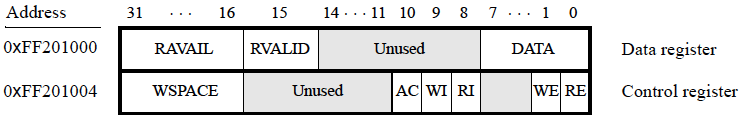
\includegraphics[scale=0.55]{figures/figureJTAG.png}
	\end{center}
	\caption{Registers in the JTAG UART interface.}
\label{fig:jtag_port}
\end{figure}

A subroutine that sends a byte of character data to the JTAG UART is given in 
Figure~\ref{fig:JTAG}.  It first reads the JTAG UART {\it Control} register to confirm that
space is available in the FIFO, and then stores the outgoing byte into the {\it Data} register.

\begin{figure}[]
\begin{center}
\lstinputlisting[style=defaultNiosVStyle, name=JTAG, firstline=15, lastline=25, showlines=true]
{../design_files/part1.s}
\end{center}
\caption{Sending character data to the JTAG UART.}
\label{fig:JTAG}
\end{figure}

\subsection*{Part I}

Figure~\ref{fig:part1} gives an example of assembly language code that uses the Terminal
window. In Part~($a$) of the figure the main program first initializes the Nios~V stack
pointer ({\it sp}) register to a location in the main memory.  
Then, three subroutines are called in sequence, 
to ''print'' character data on the Terminal window: first, {\it puts} prints a text string,
then {\it hex\_digit} prints a single hexadecimal digit (\texttt{0xB} in this example),
and finally {\it put\_JTAG} sends a newline character to the Terminal window. After these
subroutines are called, the Terminal window will display

\begin{verbatim}
Digit value: 0xB
\end{verbatim}

\newpage
\begin{figure}[bh]
\begin{center}
\lstinputlisting[style=defaultNiosVStyle, name=JTAG_example, lastline=14, showlines=true]
{../design_files/part1.s}
\end{center}
\caption{An example of code that uses the Terminal window (Part $a$).}
\label{fig:part1}
\end{figure}

The text string \texttt{Digit value...} that is displayed on the Terminal window is specified by 
using the \texttt{.asciz} assembler directive at the bottom of Part ($b$) of 
Figure~\ref{fig:part1}. This directive places into memory the ASCII code (byte) for each 
letter in the string, terminating the string with a byte value of 0.

~\\
The {\it puts} subroutine is shown at the top of Figure~\ref{fig:part1}$b$. It receives 
a pointer to a string in argument register {\it a0}, and uses a loop to send each character 
in the string to the JTAG UART. The loop is terminated when the 0 byte at the end of the
string is reached. Note that the {\it puts} subroutine saves its return address, which is in
register {\it ra}, onto the stack before executing any nested subroutine calls to 
{\it put\_JTAG}. This saved {\it ra} value is restored from the stack before {\it puts}
executes its \texttt{ret} instruction.

~\\
The {\it hex\_digit} subroutine in Figure~\ref{fig:part1}$b$ sends a single hexadecimal
digit, which is assumed to be within the correct range of \texttt{0} to \texttt{0xF}, to
the Terminal window. Before passing the digit value to the {\it put\_JTAG} subroutine it
is converted to an ASCII code by adding the appropriate amount. ASCII codes for the numerals
\texttt{0} to \texttt{9} are \texttt{0x30} to \texttt{0x39}, respectively, and thus require 
the addition of \texttt{0x30} to the corresponding hexadecimal digit.  ASCII codes for 
the letters \texttt{A} to \texttt{F} are \texttt{0x41} to \texttt{0x46}, respectively, 
requiring the addition of \texttt{0x37} to the hexadecimal digit. 

~\\
Created a file called {\it part1.s} and enter the code from
Figures~\ref{fig:JTAG}~and~\ref{fig:part1} (enter the main program code first, and then
the rest of the code). Execute this code and ensure that you fully understand how it works.

\begin{center} \begin{minipage}[h]{15 cm}
\lstinputlisting[style=defaultNiosVStyle, name=JTAG_example, firstnumber=last,
firstline=27]{../design_files/part1.s}
\end{minipage} \end{center}
\begin{center}
Figure~\ref{fig:part1}. An example of code that uses the Terminal window (Part {\it b}).
\end{center}

\subsection*{Part II}

In Part I we used the subroutine {\it hex\_digit} to display a single hexadecimal digit on 
the Terminal window. In this part you are to use the same code as for Part I, but instead of 
calling the {\it hex\_digit} subroutine you should call a new subroutine named {\it hex\_word}.
This subroutine, which you are to write, should display all eight digits in a hexadecimal
word of data on the Terminal window. Your {\it hex\_word} subroutine should receive its
argument in register {\it a0}. As an example, if {\it dec\_word} is called with the
parameter {\it a0} = \texttt{0xBEEF}, then the Terminal window should display

\begin{verbatim}
Word value: 0x0000BEEF
\end{verbatim}

Put your code in a file called {\it part2.s} and then debug and test your solution with
various word values. 

\newpage
\subsection*{Part III}

Repeat Part II, except that instead of calling your subroutine named {\it hex\_word} you are to
call a new subroutine named {\it dec\_word}. 
This subroutine, which you are to write, should display a word of data in decimal (base 10).
Your {\it dec\_word} subroutine should receive its argument in register {\it a0}. As an example,
if {\it dec\_word} is called with the parameter {\it a0} = \texttt{0xBEEF}, then the 
Terminal window should display

\begin{verbatim}
Word value: 48879 
\end{verbatim}

Notice that leading zeros are suppressed in the above output. This feature is not
absolutely necessary, but it is a good one to include in your solution. 
Put your code in a file called {\it part3.s} and then debug and test your solution with
various word values. 

\subsection*{Part IV}

In this part you are to utilize most of the code from previous parts of the exercise, 
including the {\it hex\_word} and {\it dec\_word} subroutines that you wrote for Parts~II
and~III.  Your solution for this part of the exercise should be able to display on the
Terminal window the current value of any of the Nios~V {\it save} registers {\it s0}, {\it s1}, to
{\it s11}. The specific register that is displayed at any given time is determined by the
{\it SW} slide switches and {\it KEY} pushbuttons on the DE1-SoC board. These I/O ports
were introduced in Laboratory Exercise 3. 

~\\
As an example, register {\it s5} can be selected for display 
by setting the {\it SW} switches to provide the value \texttt{101}. Assume
that the current value in this register is $s5$ = \texttt{0x65}. Now, if {\it KEY}$_0$ is 
pressed, then the Terminal window should display the value of {\it s5} in hexadecimal, as in:

\begin{verbatim}
Contents of s5: 0x00000065
\end{verbatim}

If {\it KEY}$_1$ (or any KEY other than {\it KEY}$_0$) is pressed, then the Terminal window 
should display the value of {\it s5} in decimal, as in:

\begin{verbatim}
Contents of s5: 101
\end{verbatim}

A skeleton for the main program is provided in Figure~\ref{fig:skel}. It executes in an 
endless loop so that any save register can be selected with the {\it SW} switches 
and displayed in either hexadecimal or decimal by pressing the {\it KEY} pushbuttons.

~\\
The subroutine
{\it get\_reg}, which you are to write, receives the parameter {\it a0} = {\it SW}. It returns,
in {\it a0}, the current value of the selected {\it save} register. So, if {\it SW} is set 
to \texttt{101}, then {\it get\_reg} returns the contents of register {\it s5}.
{\it Hint}: One way to obtain the current value of the required {\it save} register in 
{\it get\_reg} is to first store all of the save registers into memory, for example on the 
stack, and then to retrieve the required register value by using the parameter {\it SW} as 
an index into the memory where the registers have been saved.

~\\
Make a new file named {\it part4.s}, fill in the missing parts of the code, and test and debug your
solution. 

\begin{figure}[t]
\begin{center}
\lstinputlisting[style=defaultNiosVStyle, name=skel, escapechar=|]{../design_files/part4.s}
\end{center}
\caption{Skeleton of main program for Part IV.}
\label{fig:skel}
\end{figure}

\input{\CommonDocsPath/copyright.tex}
\end{document}
\end{document}
